\documentclass[12pt, twoside]{article}
\usepackage[letterpaper, margin=1in, headsep=0.5in]{geometry}
\usepackage[english]{babel}
\usepackage[utf8]{inputenc}
\usepackage{amsmath}
\usepackage{amsfonts}
\usepackage{amssymb}
\usepackage{tikz}
%\usetikzlibrary{quotes, angles}

\usepackage{graphicx}
\usepackage{enumitem}
\usepackage{multicol}

\usepackage{fancyhdr}
\pagestyle{fancy}
\fancyhf{}
\renewcommand{\headrulewidth}{0pt} % disable the underline of the header

\fancyhead[RE]{\thepage}
\fancyhead[RO]{\thepage \\ Name: \hspace{3cm}}
\fancyhead[L]{BECA / Dr. Huson / 10th Grade Geometry\\* Unit 1 Intro to Geometry\\5 Sept 2019}

\begin{document}
\subsubsection*{1-1 Homework: Applying Algebra to Geometric Situations}
  \begin{enumerate}


  \item In the following two problems, solve for the value of $x$.
  \begin{multicols}{2}
    \begin{enumerate}
      \item   $x-5=12$ \vspace{6cm}
      \item   $13-x=-3$ \vspace{6cm}
    \end{enumerate}
  \end{multicols}
    \vspace{3cm}

  \item Given $g(x)=x^2-5x+15$. Simplify $g(0)$. \vspace{3cm}
  \item Given $f(x)=3x-2$. Solve for $x$ such that for $f(x)=13$. \vspace{4cm}
  \item Given $h(x)=x^2-x-12$. Solve $h(x)=0$. \vspace{5cm}
  

  \item Simplify each expression. (Leave it in radical form if necessary, not a decimal.)
    \begin{enumerate}
      \begin{multicols}{2}
      \item   $\sqrt{25}$ \vspace{1.5cm}
      \item   $\sqrt{24}$ \vspace{1.5cm}
      \end{multicols}
    \end{enumerate}
    \vspace{0.5cm}

\newpage

\item The line $l$ has the equation $y=\frac{3}{2}x-1$. 
\begin{enumerate}
  \item Write down it's slope. $m=$
  \vspace{0.5cm}
  \item Write down it's $y$-intercept. $b=$
  \vspace{0.5cm}
  \item Is the point $(4, 4)$ on the line $l$? Justify your answer.
\end{enumerate}
\vspace{2.5cm}

\item On the grid below, graph the line $y=-\frac{1}{2}x+2$.
  \vspace{0.5cm}

    \begin{center} %4 quadrant regents grid w T-Chart
    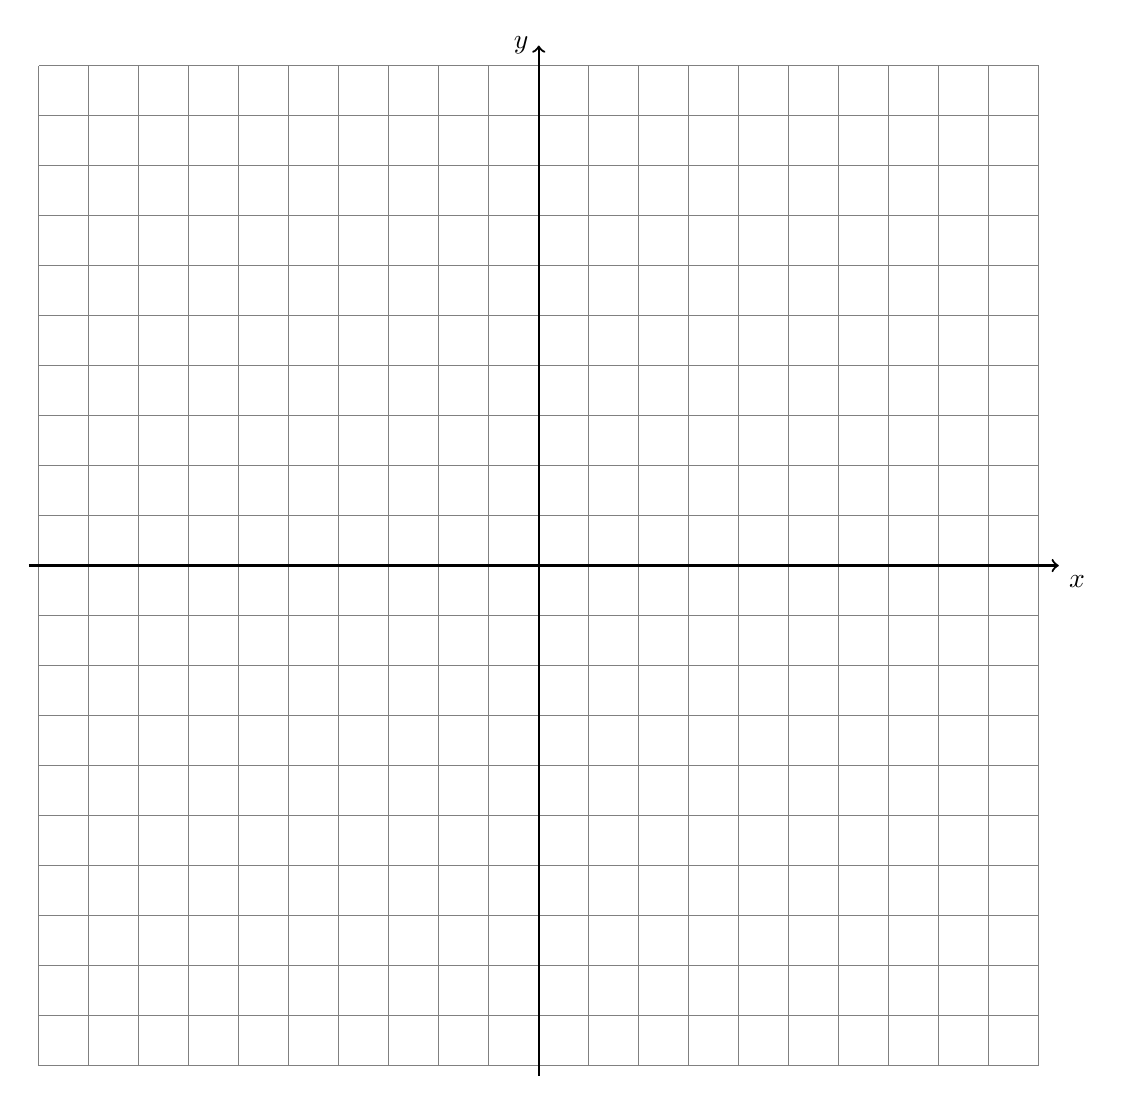
\begin{tikzpicture}[scale=.635]
      \draw [help lines] (-10,-10) grid (10,10);
      \draw [thick, ->] (-10.2,0) -- (10.4,0) node [below right] {$x$};
      \draw [thick, ->] (0,-10.2)--(0,10.4) node [left] {$y$};
    \end{tikzpicture}
    \end{center}

\end{enumerate}

\end{document}



\item As shown below, what is the translation that maps the point $R(-3,2)$ onto the point $S(6, 5)$?
\begin{center} %4 quadrant regents grid
  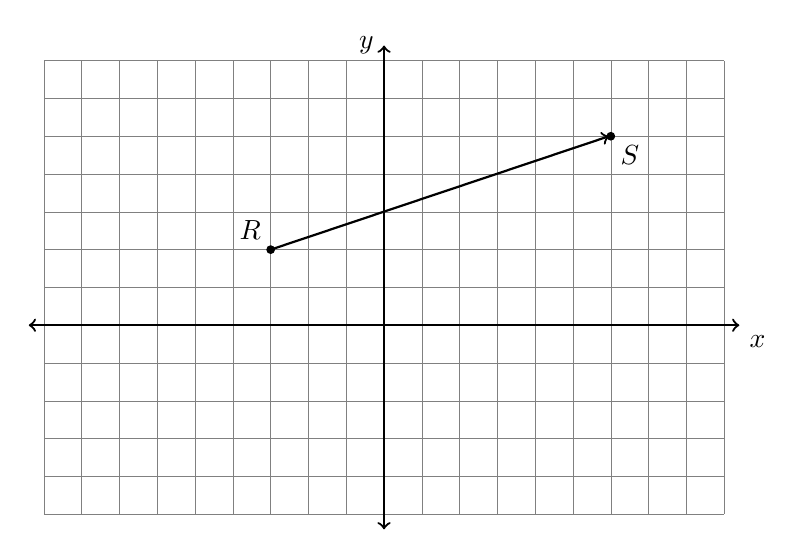
\begin{tikzpicture}[scale=.48]
    \draw [help lines] (-9,-5) grid (9,7);
    \draw [thick, <->] (-9.4,0) -- (9.4,0) node [below right] {$x$};
    \draw [thick, <->] (0,-5.4)--(0,7.4) node [left] {$y$};
    \draw [thick, ->] (-3,2)--(5.95, 5);
    \draw [fill] (-3,2) circle [radius=0.1] node[above left] {$R$};
    \draw [fill] (6, 5) circle [radius=0.1] node[below right] {$S$};
  \end{tikzpicture}
\end{center}
If only one third of that translation was performed, what coordinates would $R$ be mapped to? \vspace{2cm}
